%tusenronde 3
\begin{center}
\fbox{\fbox{\parbox{5.5in}{\centering
Schrijf hier uw antwoorden op. Er ook zijn notitie bladeren meegegeven.}}}
\end{center}
 
\vspace{5mm}
 
\makebox[\textwidth]{Teamnaam:\enspace\hrulefill}
 
\vspace{5mm}
 
\makebox[\textwidth]{Teamnummer:\enspace\hrulefill}
\section{Tafel ronde 3: raadsel ronde}
\begin{questions}
\question[2] {\begin{flushleft}
{\large Raadsel 1: Twenty-one}
\end{flushleft} 
Dit raadsel komt van de thuisstad van Tibo (cultuur home Astrid). In Koksijde staan er veel wetgevingen op hoogte bouw, dus is er maar één echt super hoog gebouw: de Twenty-one. Rara-ra, het heeft 21 verdiepen. Nu woont meneer Wesley op de 21ste verdieping. Elke dag als het mooi weer is neemt hij de lift naar beneden en de trap naar boven. Echter wanneer het slecht weer is neemt hij de lift naar beneden en ook de lift naar boven.}
\linebreak
De vraag is, hoe komt dit? Waarom neemt hij niet altijd de lift?
\linebreak
\it Hint: op slechte dagen neemt hij een paraplu mee!
\fillwithlines{\stretch{1}}
%raadsel 2
\question[1]{\begin{flushleft}
{\large Raadsel 2: Vogel}
\end{flushleft} Teken een vogel door 2 rechte strepen te plaatsen.\center

\includegraphics[scale=1]{kip}}
\newpage
\question[1] {\begin{flushleft}
{\large Raadsel 3: Symbolen}
\end{flushleft}
Bepaal de volgende symbolen (mintens 2 aanvullen ,maar maximum 5).
\center
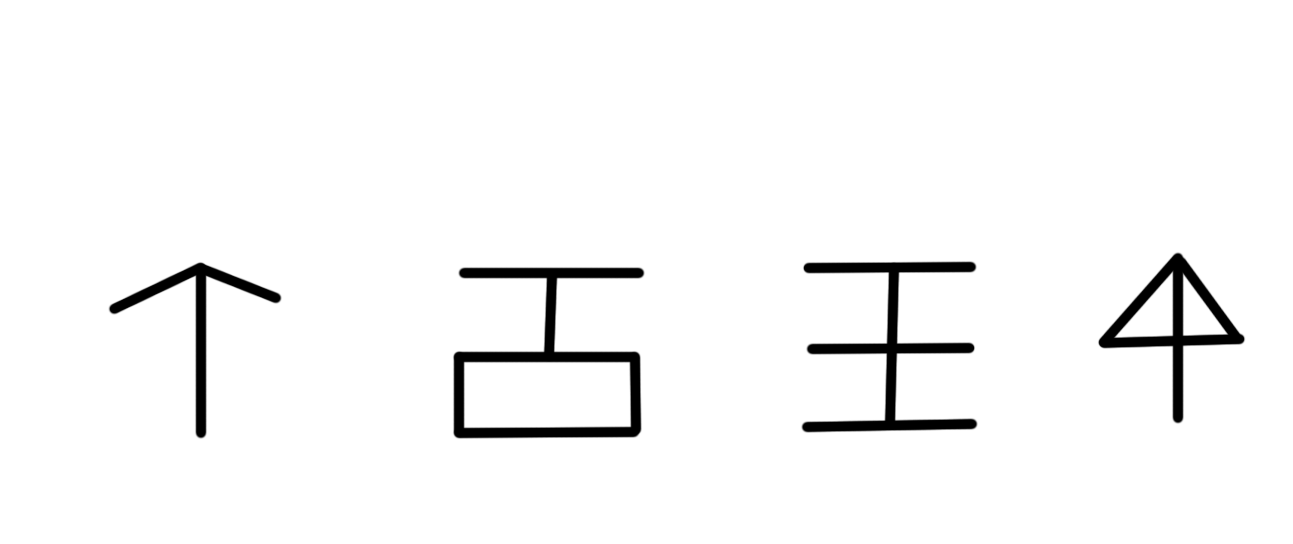
\includegraphics[scale=1]{symbolen}
}
\vspace{\stretch{1}}
\question[1] {\begin{flushleft}
{\large Raadsel 4: Ontcijfer}
\end{flushleft}
\begin{flushleft}
Ontcijfer deze boodschap!
\end{flushleft}
\begin{center}
Oleacahoydnebp xef 3
\end{center}
\it Hint! Kijk naar het nummer van het raadsel!}
\newpage
\question[1]{\begin{flushleft}
{\large Raadsel 5: converteer het symbool naar een decimaal getal.}
\end{flushleft}
\begin{center}
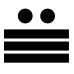
\includegraphics[scale=0.2]{76}
\end{center}
}
\end{questions}
\begin{table}[!b]
\centering
\begin{tabular}{|l|l|l|l|l|l|l|l|l|l|l|}
\hline
Vraag       & 1 & 2 & 3 & 4 & 5 & 6 & 7 & 8 & 9 \\ \hline
max. punten & 2 & 1 & 1 & 1 & 1 & 1 & 1 & 1 & 1 \\ \hline
score       &   &   &   &   &   &   &   &   &   \\ \hline
\end{tabular}
\end{table}